%\documentclass[11pt]{book}

\documentclass[10pt]{article}
\usepackage{graphicx}
\usepackage{amssymb}
\usepackage{epstopdf}
\usepackage{caption}
\usepackage[fleqn]{amsmath}
\usepackage{tipx}
\usepackage{tipa}
\usepackage{breakcites}

%\usepackage{/usr/local/texlive/2020/texmf-dist/tex/latex/breakcites/breakcites}

%\usepackage{supertabular}
%\usepackage{wasysym}

%\usepackage{setspace}
%\usepackage{/usr/local/texlive/2020/texmf-dist/tex/latex/setspace/setspace}

%\usepackage{pifont}

\usepackage{enumitem}
\usepackage{float}

%\usepackage{mathabx}

%\usepackage{/usr/local/texlive/2020/texmf-dist/tex/latex/mathabx/mathabx}

%\usepackage{txfonts}

%\usepackage{Sweave}

\usepackage{fancyvrb} %%% for \VerbatimInput

%%%%%%%%%%%%%%%%%%%%%%%% FOR HYPER REF
\usepackage{color}
\definecolor{MyDarkGreen}{rgb}{0.0,0.4,0.0}
\definecolor{MyDarkRed}{rgb}{0.4,0.0,0.0} 
\definecolor{MyBlue}{rgb}{0.0, 0.0, 0.5} 
\definecolor{MyOrange1}{rgb}{1.0, 0.9, 0.0} 
\usepackage[colorlinks=true, urlcolor= MyDarkRed, linkcolor= MyBlue, citecolor=MyDarkGreen ]{hyperref}

%\usepackage[colorlinks=false, urlcolor= MyOrange1, linkbordercolor=MyOrange1, citecolor=MyDarkGreen ]{hyperref}

\usepackage{makeidx}

%\usepackage[colorlinks=true, urlcolor= \rgb{0.0,0.2,0.0}  ]{hyperref}
%EG -- in document
%\url{http://www.stat.ucla.edu/~davezes/CES/LE_cost_Full.mov}
%\singlespacing
%\onehalfspacing
%\doublespacing
%\pagestyle{empty} %% turn off page numbering

\DeclareCaptionLabelSeparator{space}

\DeclareGraphicsRule{.tif}{png}{.png}{`convert #1 `dirname #1`/`basename #1 .tif`.png}
\textwidth = 7.5 in
\textheight = 9.2 in
\oddsidemargin = -0.5 in
\evensidemargin = -0.5 in
\topmargin = -0.5 in
\headheight = 0.0 in
\headsep = 0.2 in
\parskip = 0.2in
\parindent = 0.0in
\newtheorem{theorem}{Theorem}
\newtheorem{corollary}[theorem]{Corollary}
\newtheorem{definition}{Definition}

%\title{Brief Article}
%\author{The Author}

\setcounter{secnumdepth}{3}
\setcounter{tocdepth}{3}

\makeindex

\begin{document}

%\maketitle

\newif\ifuselocaldir
\uselocaldirtrue
\uselocaldirfalse

\newcommand{\DXZ}{
\begin{flushright}
\vspace{-.4in}
 { \raisebox{0.30ex}{{\tiny D}}\hspace{0.008in}X\hspace{0.01in}\raisebox{0.30ex}{{\tiny Z}}     }
\end{flushright}
}

\newenvironment{myQuote}[2]%
               {\begin{list}{}{\leftmargin#1\rightmargin#2}\item{}}%
               {\end{list}}

\begin{myQuote}{4cm}{4cm}
\begin{center}
{\huge
\textbf{IMDb Analysis} \\[0.4cm]
}
{\Large
MAS 405 S2022
}
\end{center}
\end{myQuote}

%\begin{myQuote}{3cm}{3cm}
%\begin{center}
%PRILIMINARY \& INCOMPLETE \\
%\end{center}
%\end{myQuote}

\begin{myQuote}{3cm}{3cm}
{\normalsize
\begin{center}
Sofia Alcazar, Dylan Jorling, Daniel Kwon, Andrew Mashhadi, Ajay Patel \\
\today
%2012-03-12
\end{center}
}
\end{myQuote}

%\begin{abstract}
%{\normalsize
%Here's my abstract
%}
%\end{abstract}

%\newpage

%%\tableofcontents

%\newpage

%\input{_example.tex}

%\chapter{Introduction}


\begin{center}
\includegraphics[width=17cm]{_assets/moviePosterArray.jpeg}
\end{center}


\quad Congrats! You just landed a coveted job at one of the world’s greatest film production companies as an executive movie producer! No need to worry that you lack experience in producing; we can help guide you through what it takes to create an iconic movie through the analysis of historical IMDb data. There are many ways a movie can be defined as successful, and we’ll help you on each path. Are you looking to maximize box office earnings? Are you hoping to sweep award ceremonies? Maybe you’re looking to simply make a popular, household movie for years to come? We can help guide your decision, no matter the success you wish to achieve. 

\begin{center}
\section*{Opportunity}
\end{center}

\quad In our research, we found which traits and features of movies are correlated with success by breaking the analysis down into three different categories:

\begin{enumerate}
\item Maximize box office profits
\item Maximize chances of an Academy Award nomination
\item Finding movies that are similar to a specified existing film
\end{enumerate}

\begin{center}
\section*{Solutions and Recommendations}
\end{center}

\begin{center}
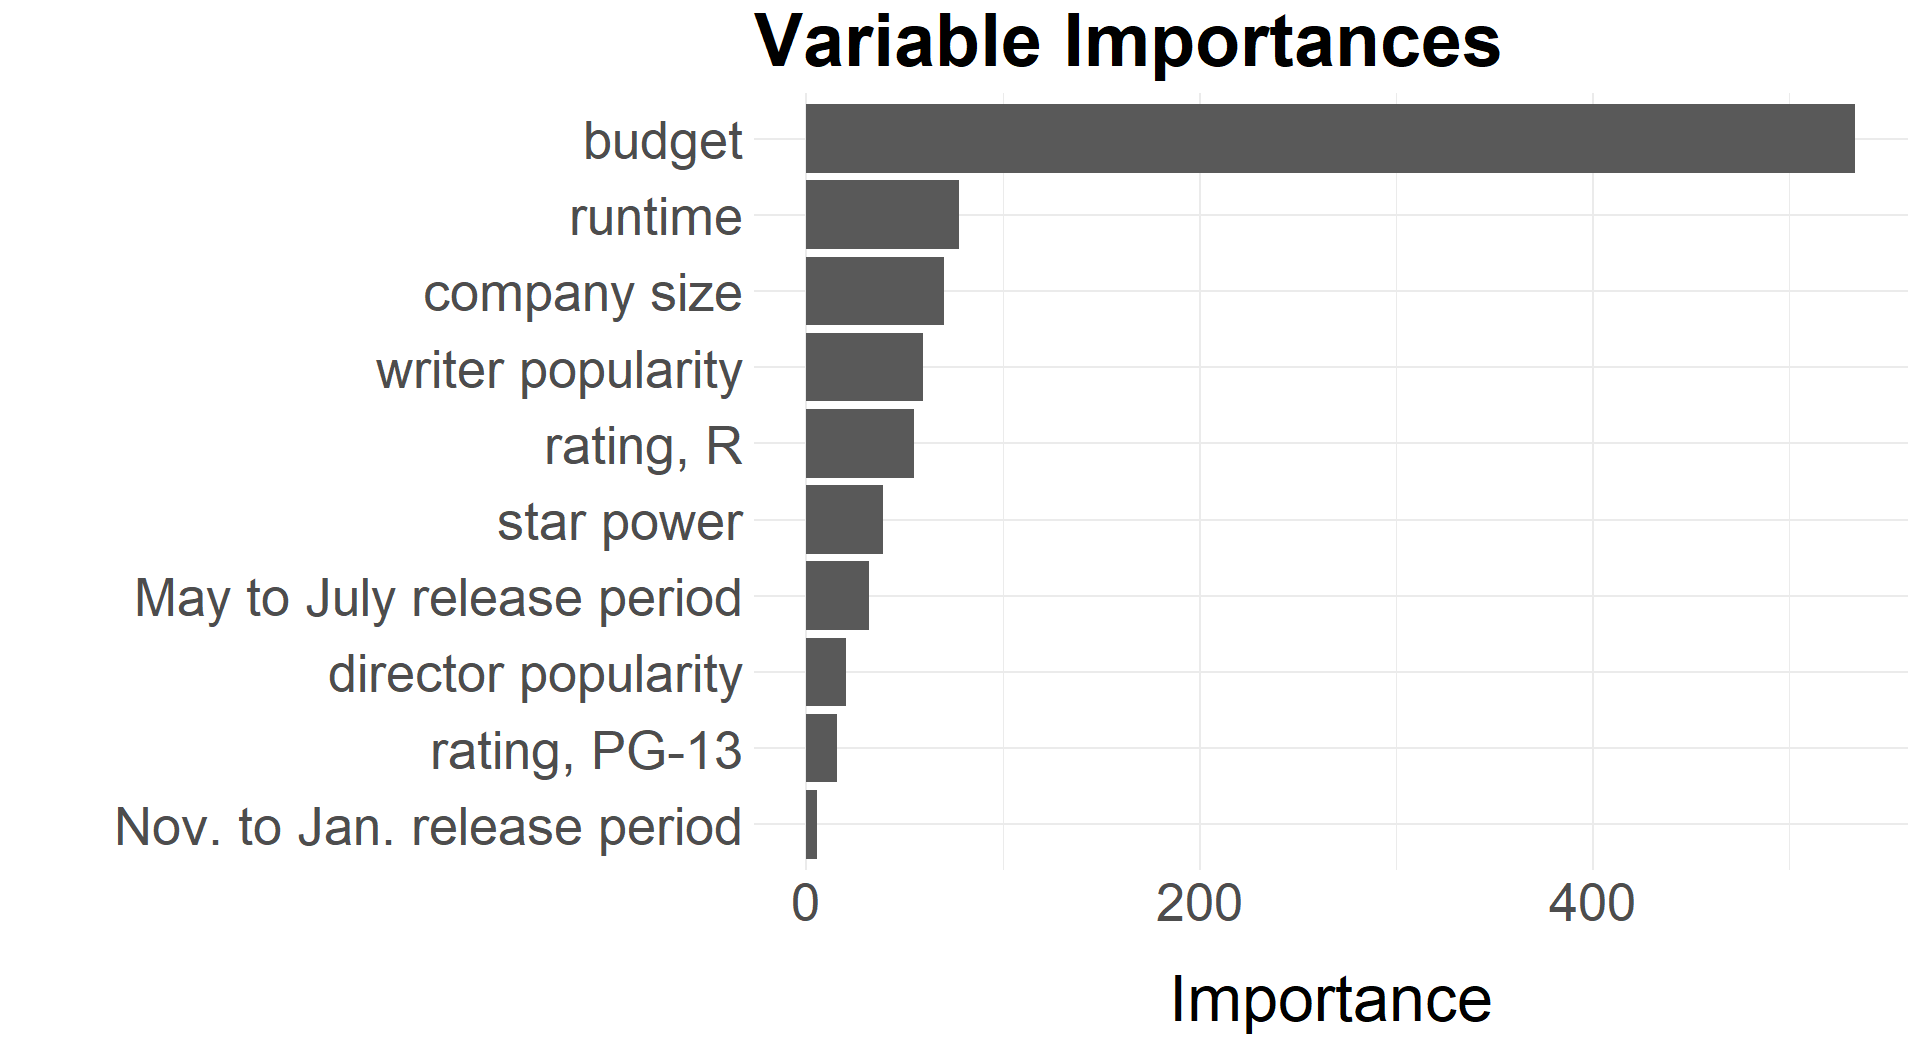
\includegraphics[width=8cm]{_assets/predictive_analysis/variable_importance_rf_bop.png}
\hspace{1cm}
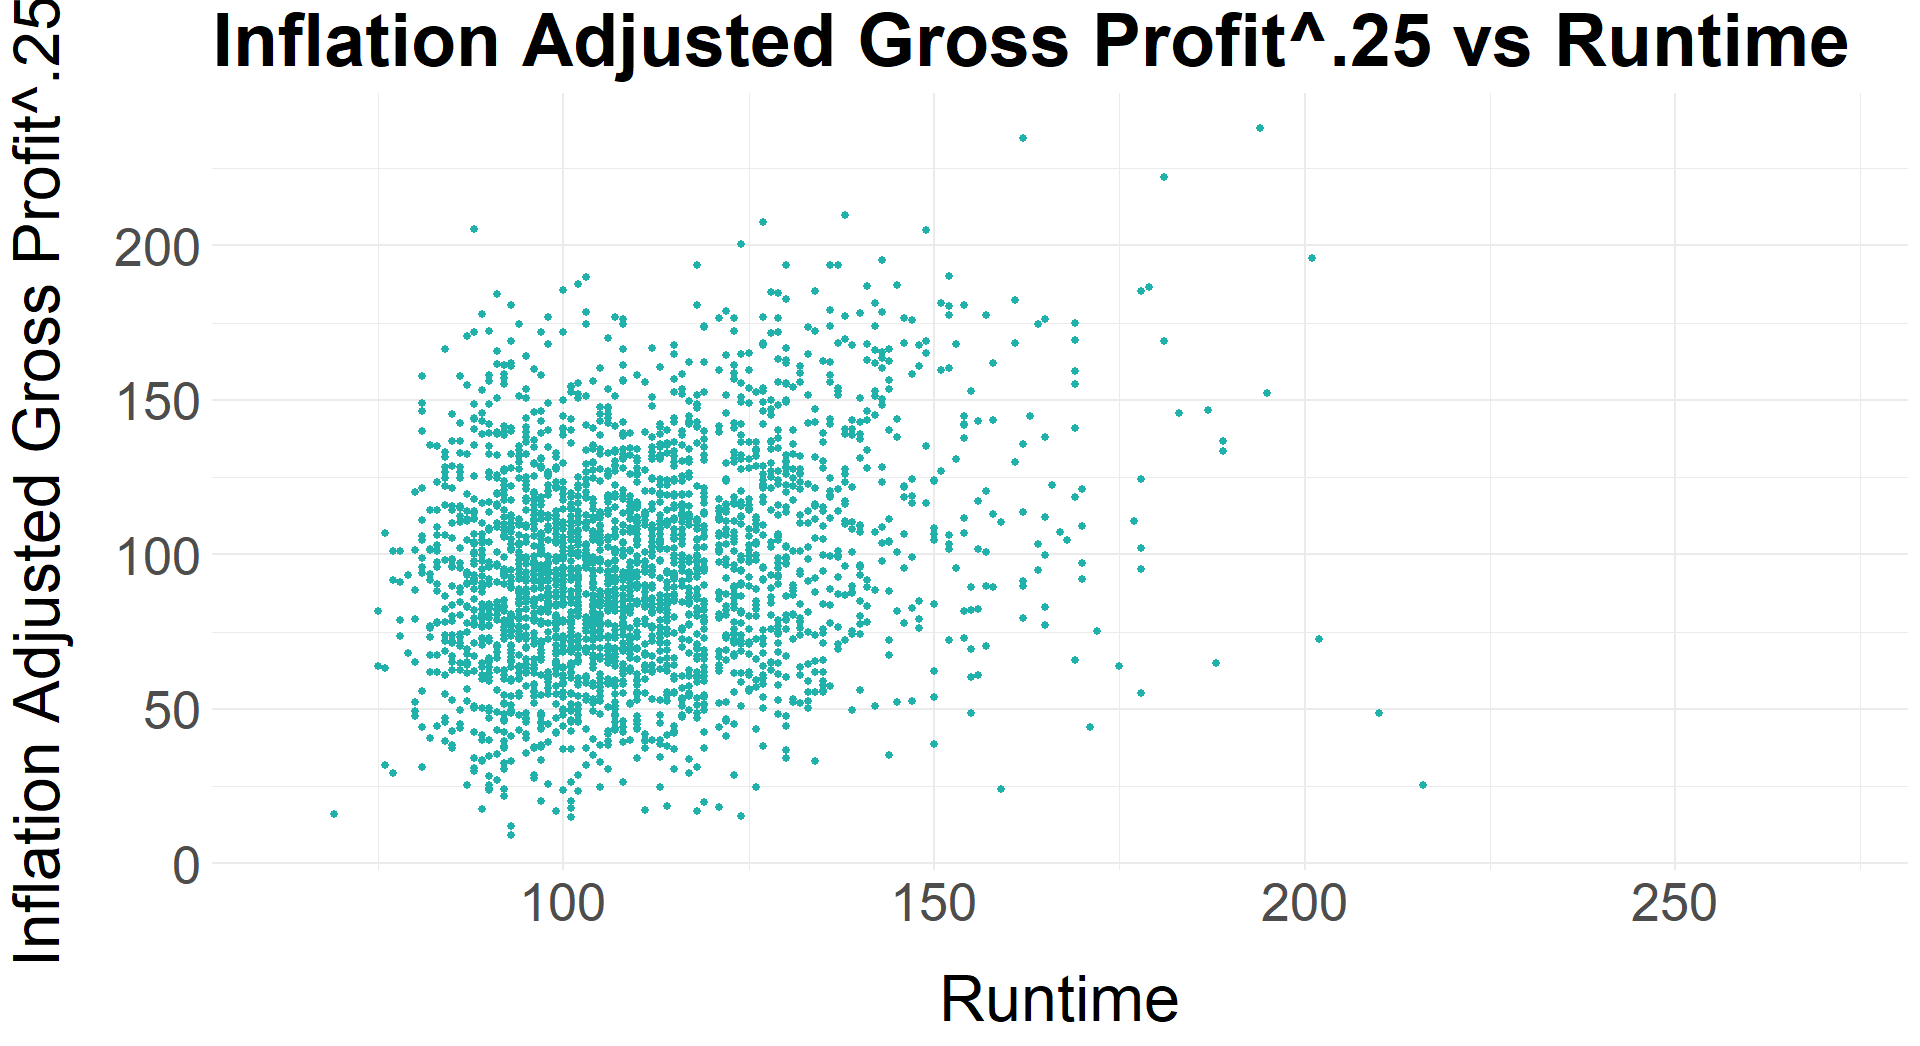
\includegraphics[width=8cm]{_assets/_eda/runtime_iagp.png}
\end{center}

\quad To address the first opportunity, maximizing box office profits, we used a random forest. Using budget, runtime, genres, content rating, director popularity, movie release period, runtime, company size, star power, and writer popularity as predictor variables, we trained our random forest algorithm. After tuning our hyper-parameters, we found that 1100 trees (bootstrap resamples) with 7 variables randomly sampled as candidates for each split were optimal for our model. From the above plot it's clear that budget has the highest feature importance. This is not surprising and means that your movie’s budget demonstrates the greatest ability to predict box office profits compared to all of the other variables used in the random forest. While budget is most important, we also found that runtime, company size, writer popularity, and R ratings demonstrate a fairly strong predictive power. All in all, we recommend a high budget movie with a longer run time and R rating to maximize box office profits. 

\begin{center}
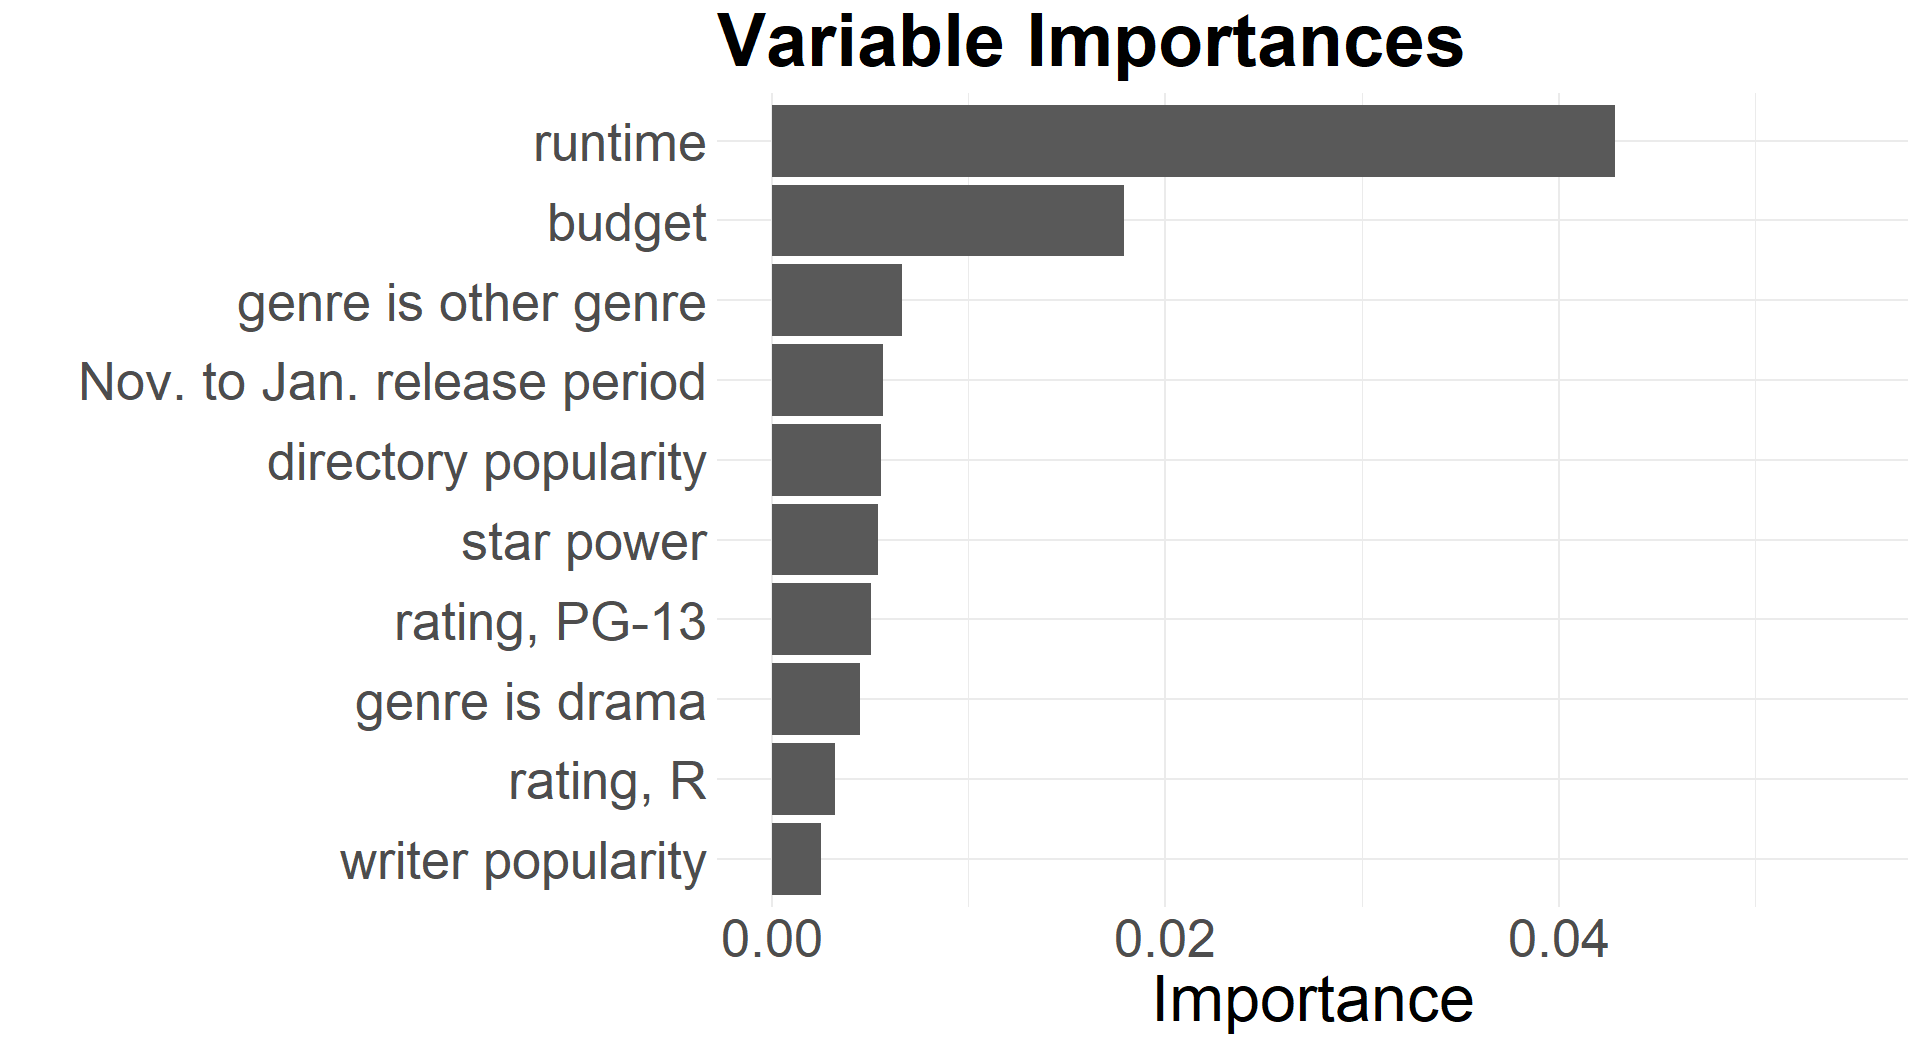
\includegraphics[width=8cm]{_assets/predictive_analysis/variable_importance_rf_osc_nom.png}
\hspace{1cm}
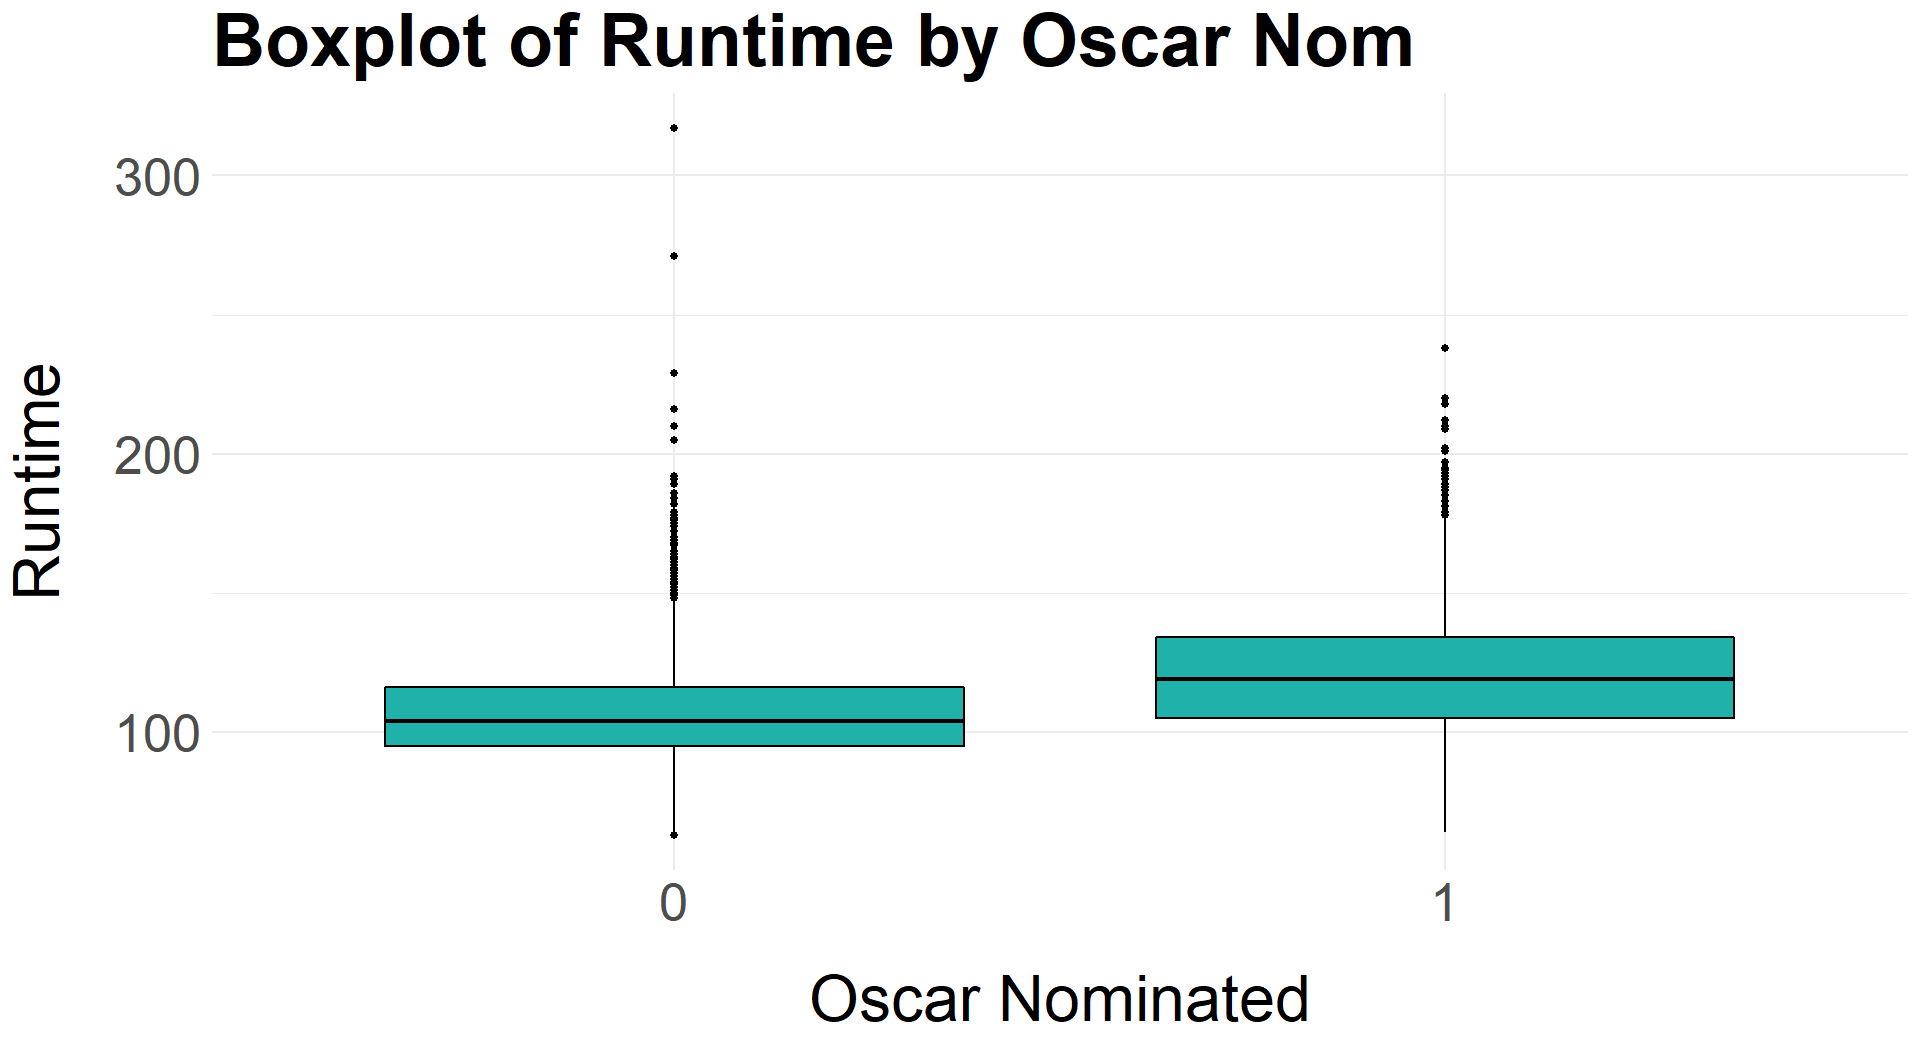
\includegraphics[width=8cm]{_assets/_eda/runtime_on.png}
\end{center}

\quad Similar to the first opportunity, we used a random forest to model the chances of an Academy Award nomination. Using budget, runtime, genres, content rating, director popularity, movie release period, runtime, company size, star power, and writer popularity as predictor variables, we trained our random forest binary classification model. For this model, we found that 1250 trees (bootstrap resamples) with 7 variables randomly sampled as candidates for each split were optimal for our model. To support this model, we also fit a logistic regression model with the same data. Ultimately, we found that runtime, budget, genre, and release period are among the most important predictors for award nominations. We recommend increasing runtime and budget, and releasing a drama film during the months of November to January to increase your chances of receiving an Academy Award Nomination.

\begin{center}
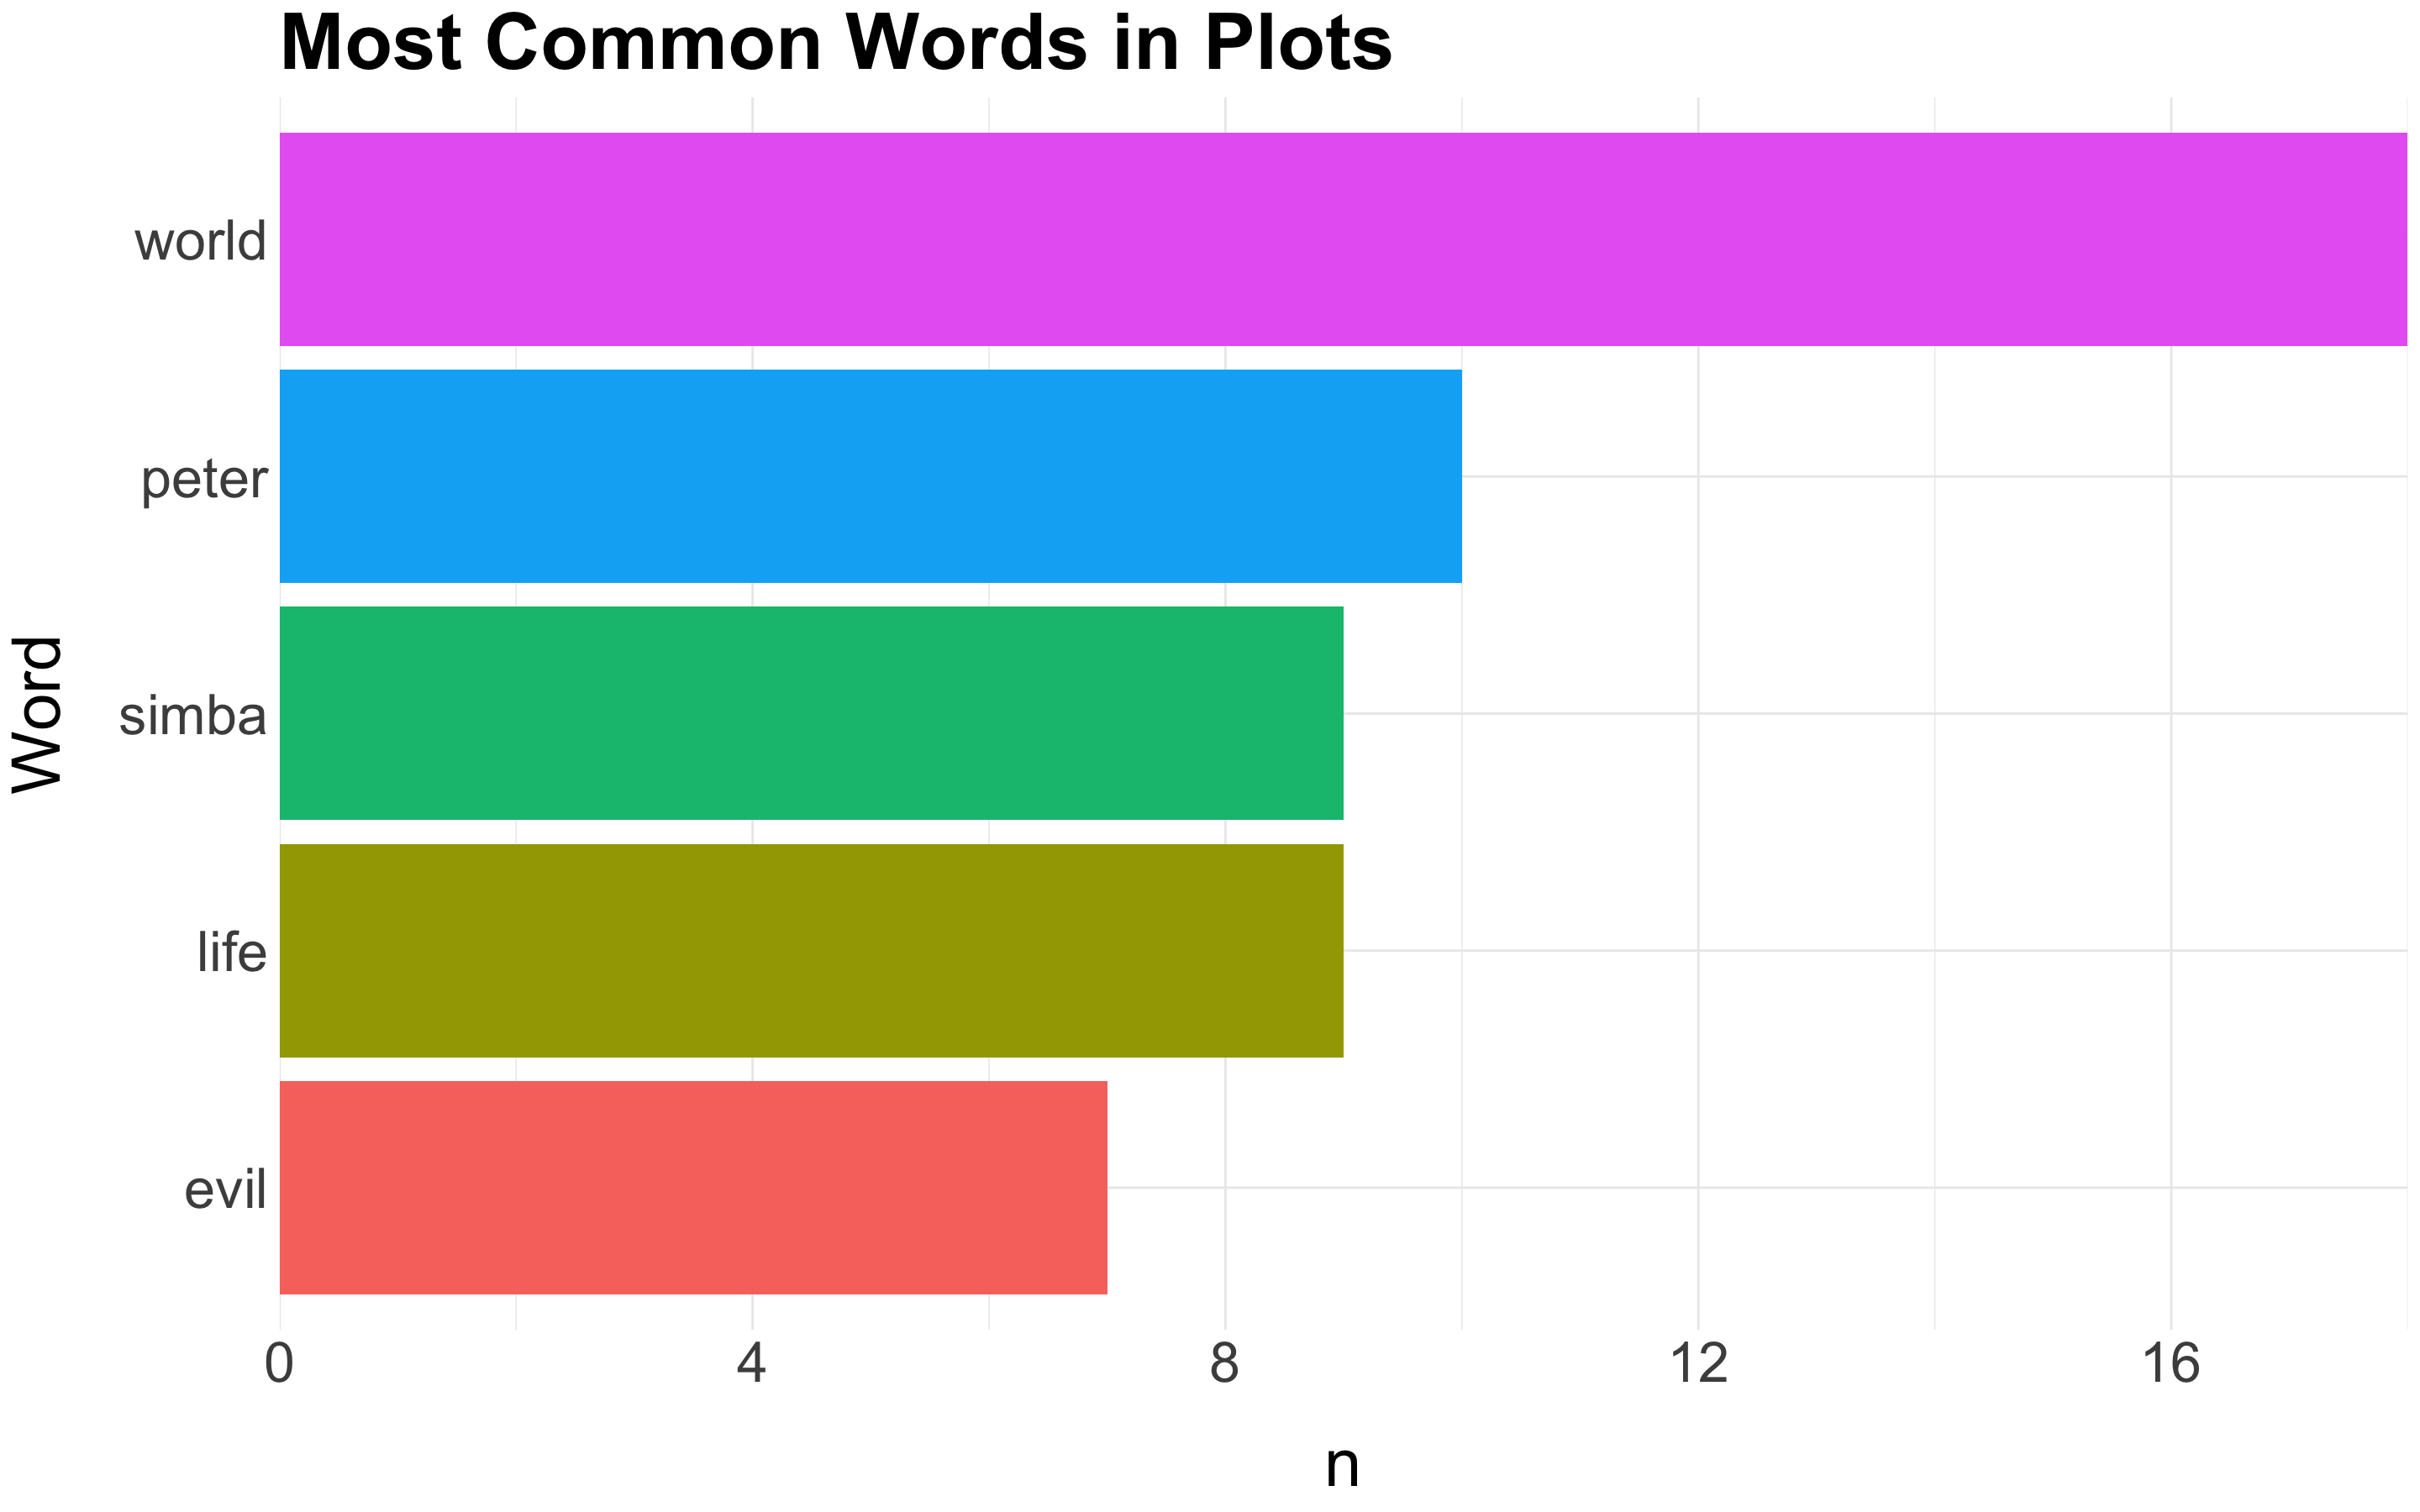
\includegraphics[width=8cm]{_assets/_assets_knn/star_wars_common_words.png}
\hspace{1cm}
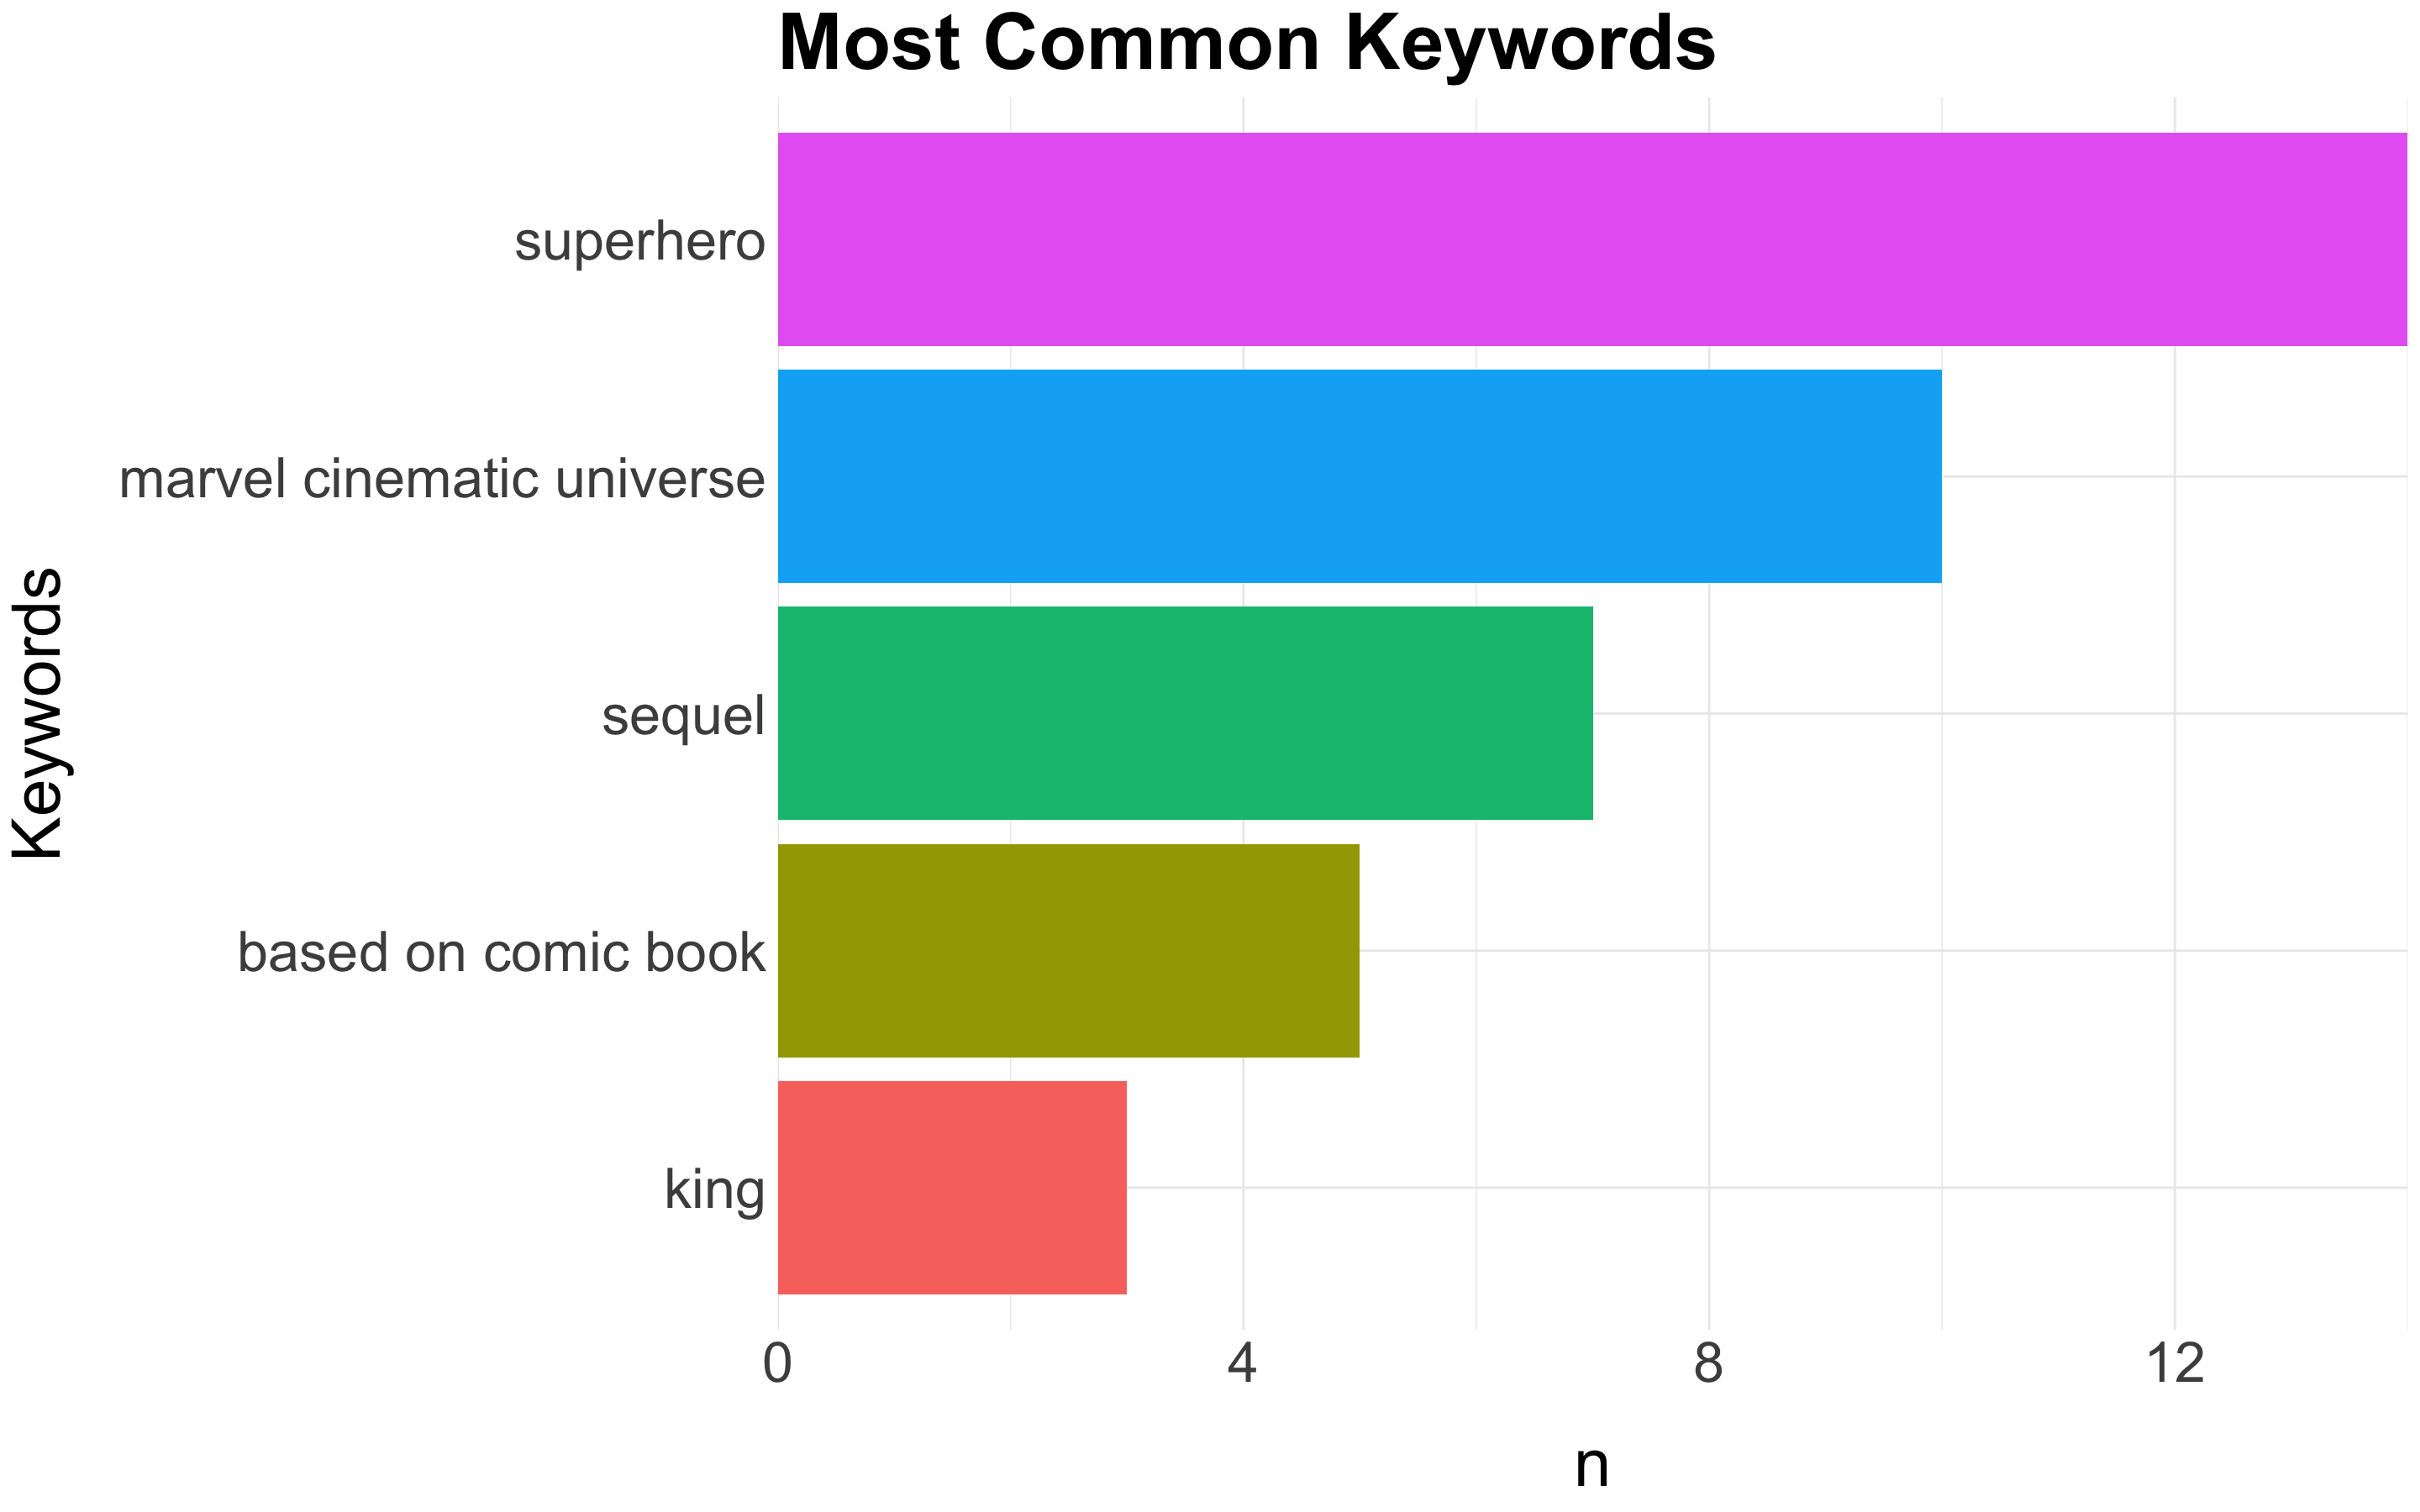
\includegraphics[width=8cm]{_assets/_assets_knn/star_wars_common_keywords.png}
% latex table generated in R 4.2.0 by xtable 1.8-4 package
% Sat Jun  4 12:47:09 2022
\begin{table}[H]
\centering
\begin{tabular}{llr}
  \hline
Full Title & Gross USA \$ & Oscar Won \\ 
  \hline
Star Wars: Episode VII - The Force Awakens (2015) & 936,662,225 &   0 \\ 
  Spider-Man: No Way Home (2021) & 804,617,772 &   0 \\ 
  Avengers: Infinity War (2018) & 678,815,482 &   0 \\ 
  Avengers: Endgame (2019) & 858,373,000 &   0 \\ 
  Incredibles 2 (2018) & 608,581,744 &   0 \\ 
  Star Wars: Episode VIII - The Last Jedi (2017) & 620,181,382 &   0 \\ 
  Black Panther (2018) & 700,426,566 &   1 \\ 
  The Lion King (2019) & 543,638,043 &   0 \\ 
  Jurassic World (2015) & 653,406,625 &   0 \\ 
  Avatar (2009) & 760,507,625 &   1 \\ 
   \hline
\end{tabular}
\caption{The Nearest Movies to Star Wars: Episode VII - The Force Awakens (2015)} 
\end{table}


\end{center}

\quad Lastly, we can leave you with a few movie recommendations that are most similar to a specified existing movie, in case you liked to mimic their success. If you want to create a movie similar to Star Wars: Episode VII - The Force Awakens (2015), we recommend that you work with Disney as other Disney movies are the most similar to Star Wars: Episode VII - The Force Awakens (2015). Also, among its 50 nearest movies, the most common word from the plot summary is “world”. This is not surprising as Marvel movies focus on a group of heroes trying to save the world from an evil being. To mimic this movie, we recommend you create a movie in the superhero action or adventure genre. If your goal is to mimic a movie that was highly nominated like The Godfather (1972), you’ll definitely want to focus on other important things. The Godfather (1972) has the highest metacritic and IMDb rating among movies that won an Oscar. We suggest that you analyze other 1970s crime films such as The Godfather: Part II (1974), Midnight Express (1978), Taxi Driver (1976), and Chinatown (1974) because these films are included in the Godfather’s 9 nearest movies. Since the majority of the nearest neighbors are drama and crime films, we also suggest the new movie include murder, revenge, and organized crime. Finally, if you love the movie Forrest Gump (1994) and would hope to mimic the onscreen magic of Tom Hanks, we suggest you look to The Great Gatsby (2013), A Beautiful Mind (2001), or Cinderella Man (2005) for inspiration. We suggest you cast the talented Leonardo DiCaprio or Russell Crowe because they’re featured in these films, as well as aim for the genre of drama or romance. 
Good luck in your new role! See you at the cinema!

 \end{document}





